%version of 02-27-19

\chapter{EXERCISES}
\label{ch:Exercises}


\section{Summation}


\subsection{Compute $\Delta_n$ and sum of squares}

\ignore{$\Delta_n = \sum_{i=1}^{n} i = \frac{n(n+1)}{2}$

Use the same technique of writing the same sum by extracting the first and the last element provides a nice example.

We loose since the coefficient of the $\Delta_n$ is the same after these manipulations, but we can manage if we compute the \textit{next} sum, that is sum of the squares.
\medskip

$\Delta_{n+1} = 1 + \sum_{i=1}^{n+1} i $

$\Delta_{n+1} = (\sum_{i=1}^{n} i) + \frac{(n+1)(n+2)}{2}$
}

\section{Tetrahedral numbers}

The sum of the $\Delta_n$ is denoted by $\Theta_n$ and it is called a tetrahedral numbers:

$\Theta_n =  \sum_{k=1}^{n} \Delta_k$.

%We can show that: $\Theta_n = \frac{n.(n+1).(n+2)}{6}$

A way to prove this expression is to consider three copies of $\Theta_n$ and organize them in order to obtain the expected result
(remember the way we established the closed formula for triangular numbers was based on $2$ copies
arranged in the right form).
The basic tetrahedral number is organized as a triangle (see Figure~\ref{fig:TetrahedralBasic}).
The proof is obtained by Fubini's principle by rotating this triangle as shows in Figure~\ref{fig:Tetrahedral}.

\begin{figure}[h]
\begin{center}
        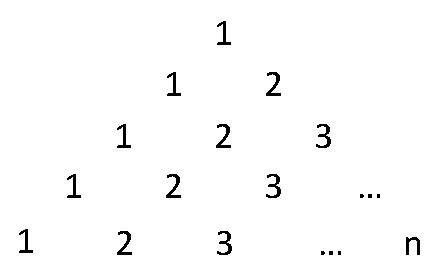
\includegraphics[scale=0.5]{FiguresArithmetic/TetrahedralBasic}
        \caption{Computing $\Theta_n$: basic triangle pattern.}
        \label{fig:Tetrahedral}
\end{center}
\end{figure}

The first row is equal to $n+2$.

The second one is equal to $3 + 2(n-1)+3 = 2(n+2)$. 

Let us sum up the elements in row $k$: 

$\Delta_k + k(n-k+1) + \Delta_k = k(k+1) +kn-k^2+k = k(n+2)$.

Thus, the global sum is equal to $n+2$ times $(1+2+...+n)$.

Finally, $3 \Theta_n = (n+2) \Delta_n$

\begin{figure}[h]
\begin{center}
        \includegraphics[scale=0.5]{FiguresArithmetic/Tetrahedral}
        \caption{Computing $\Theta_n$ using an adequate arrangement of $3$ triangles.}
        \label{fig:Tetrahedral}
\end{center}
\end{figure}

Summary and extension:

We proved some results, in particular:
\begin{itemize}
\item $Id_n = 1+1+ ... +1 = n$
\item $\Delta_n = 1+2+3+ ... +n = \frac{1}{2}.Id_n.(n+1)$
\item $\Theta_n = \Delta_1 + \Delta_2 + ... + \Delta_n = \frac{1}{3} .\Delta_n.(n+2)$
\end{itemize}

A natural question is if we can go further following the same pattern for computing $ \sum_{k=1}^{n} \Theta_k$, and so on.

\section{More exercises}

\subsection{Graphical proofs 1}

Compute sum of squares with 3 copies and fill the 2D rectangle. 
We should add here the figures that have been removed from the chapter SUMMATION. 

\subsection{Graphical proofs 2}

Computing the sum of $(\frac{1}{4})^k =\frac{1}{3} $ using a graphical argument.

The solution is depicted in Fig.~\ref{Fig:SUmgeo1sur4}. 


\begin{figure}
\begin{center}
        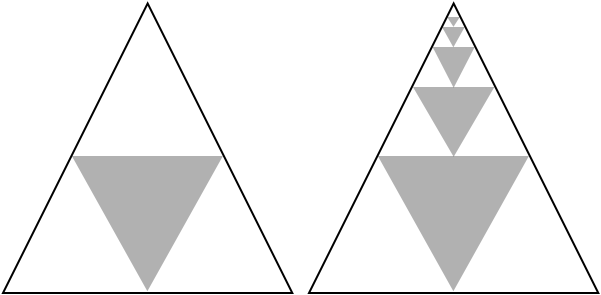
\includegraphics[scale=0.4]{FiguresArithmetic/SumGeometric1sur4}
        \caption{Graphical construction. Assuming the total surface is 1, the surface of the the internal triangle (in blue) is $\frac{1}{4}$.
        As the blue surface is one third at each layer, the global surface is $\frac{1}{3}$.
        By Fubini principle, this surface is the sum of the $\frac{1}{4^k}$ (for $k \geq 1$).}
        \label{Fig:SUmgeo1sur4}
\end{center}
\end{figure}


\subsection{Harmonic series}

$H_{n} = \sum_{k=1}^{n} \frac{1}{k}$.

Another way to prove that the sum is infinite:
 
The analysis is as follows.
Group the terms according to powers of $2$. 
The sum within each group is between $\frac{1}{2}$ and $1$, thus,
$H_n > \frac{1}{2}.n$
\\

Another (more precise) way is to gather the terms 3 by 3 as follows:

$S_k = (\frac{1}{3k-1} + \frac{1}{3k} + \frac{1}{3k+1} )$ for $k\geq1$, 

$H = 1 + S_1 + ... + S_k + ... > 1 + 3.\frac{1}{3} + 3.\frac{1}{6} + ... + 3.\frac{1}{3k} + ... $

since $S_k > 3.\frac{1}{k} $.

The proof is by contradiction, if $H$ is finite, from the previous relation we have: $H > 1 + H$, which is obviously impossible.
\bigskip

Moreover, the first way of  bounding the sum tells us about its value (actually, we know the value at a factor of $2$):

$\frac{log(n)+1}{2} < H_n < log(n)+1$. Thus, $H_n = \O(log(n))$



\section{Arithmetic}

\subsection{A fun result: complex
  multiplication via $3$ real multiplications}
\index{complex number!multiplication via 3 real multiplications}

\begin{prop}
%\label{thm:complex-mult-3real}
One can compute the product of two complex numbers using {\em three}
real multiplications rather than four.
\end{prop}

\begin{proof}
Although implementing (\ref{eq:complex-mult}) ``directly'' correctly
produces the product $\kappa = (a+bi) \cdot (c+di)$, there is another
implementation that is {\em more efficient}.  Specifically, the
following recipe computes $\kappa$ using only {\em three} real
multiplications instead of the four real multiplications of the
``direct'' implementation.  We begin to search for this recipe by
noting that our immediate goal is to compute both Re$(\kappa) = ac-bd$
and Im$(\kappa) = ad+bc$.  We can accomplish this by computing the
{\em three} real products
\begin{equation}
\label{eq:complex-mult-3a}
(a+b) \cdot (c+d); \ \ \ \ \
ac;  \ \ \ \ \ bd
\end{equation}
and then noting that
\begin{equation}
\label{eq:complex-mult-3b}
\begin{array}{lcl}
\mbox{Im}(\kappa) & = & (a+b) \cdot (c+d) - ac -bd, \\
\mbox{Re}(\kappa) & = & ac -bd
\end{array}
\end{equation}
We thereby achieve the result of the complex multiplication described
in (\ref{eq:complex-mult}) while using only {\em three} real
multiplications.

Of course, a full reckoning of the costs of the two implementations we
have discussed exposes the fact that the implementation that invokes
(\ref{eq:complex-mult-3a}) and (\ref{eq:complex-mult-3b}) uses {\em
  three} real additions rather than the {\em two} real additions of
the ``direct'' implementation.  But this entire exercise was
predicated on the observation that each real addition is much less
costly than a real multiplication, so trading one multiplication for
one addition is an unqualified ``win''.  \qed
\end{proof}

Extension of the same method: 

Notice that this technique is classical and it has been used in many other situations.
For instance while multiplying two integers in base 2 (see exercice~{Karatsuba}).




\subsection{A Fun Result: A ``Trick'' for Squaring Certain Integers}

Sometimes only basic knowledge is needed to craft amusing
``tricks''---we know that they are not really tricks at all!---that
are really rigorous applications of principles that we have learned.
Here is an ``old chestnut'' example that may inspire you to design
your own. 

If someone presents you with a number that has a numeral that ends in
$5$, then there is a simple way to square the number mentally.  For
instance, if someone says

\hspace{.25in}``$n = 25$''

\noindent
then you can instantly respond

\hspace{.25in}``$n^2 = 625$''

\noindent
If the challenge is

\hspace{.25in}``$n = 75$''

\noindent
then your response is

\hspace{.25in}``$n^2 = 5625$''

\noindent
Let's make this ``game'' mathematical.

\begin{prop}
\label{thm:75x65=4925}
Let $n$ be any number that has a $2$-digit decimal numeral of the form

\hspace{.25in}$\delta \ 5$ \ \ \ \ $(\delta \in \{ 0,1,2,3,4,5,6,7,8,9\})$.

\noindent
Then the square of $n$ is the integer

\hspace{.25in}$25 \ + \ \delta \cdot (\delta +1)$. 
\end{prop}

\begin{proof}
We can rewrite the premise of the proposition in the form
\[ n \ = \ 10 \cdot \delta + 5 \]
It is now easy to invoke Proposition~\ref{prop:(a+b)(c+d)} and the
distributive law to compute that

\[ n^2 \ = \ 100 \cdot \delta \cdot (\delta+1) + 25. \]
To wit: 
\[
\begin{array}{lclll}
n^2 & = & (10 \cdot \delta + 5)^2 & & \mbox{Given} \\
    & = & 100 \cdot \delta^2 \ + \ 100 \cdot delta \ + \ 25
              & & \mbox{the proposition} \\
    & = & 100 \cdot (\delta^2 \ + \ \delta) \ + \ 25
              & & \mbox{factoring: distributive law} \\
    & = & 100 \cdot \delta \cdot (\delta + 1) \ + \ 25
              & & \mbox{factoring: distributive law} \\
\end{array}
\]
A parlor trick has become a mathematical demonstration!
\qed
\end{proof}


\subsection{A fun result via geometric sums: When is integer  $n$
  divisible by $9$?}
\label{sec:divisible-by-9}

We now exploit our ability to evaluate geometric summations to
illustrate a somewhat surprising, nontrivial fact.  One can deduce
information about the divisibility of an integer $n$ from $n$'s
positional numerals.  We hope that this ``fun'' result will inspire
the reader to seek kindred numeral-encoded properties of numbers.

\begin{prop}
\label{thm:div-by-b-bar}
An integer $n$ is divisible by an integer $m$ if, and only if, $m$
divides the sum of the digits in the base-$(m+1)$ numeral for $n$.
\end{prop}

The most familiar instance of this result is phrased in terms of our
traditional use of base-$10$ (decimal) numerals. \\
{\it An integer $n$ is divisible by $9$ if, and only if, the sum of
  the digits of $n$'s base-$10$ numeral is divisible by $9$.}

\smallskip

\begin{proof}
({\it Argument for general number-base $b$}).
%
Of course, we lose no generality by focusing on numerals without
leading $0$'s, because leading $0$'s do not alter a numeral's sum of
digits.

Let us focus on the base-$b$ numeral for a number $n$ (so $b = m+1$ in
the statement of the proposition).  There therefore exist base-$b$
digits---i.e., integers from the set $\{0, 1, \ldots, b-1\}$---call
them $\delta_k \neq 0$, $\delta_{k-1}$, \ldots $\delta_1$, $\delta_0$,
such that
\[ n \ = \ \delta_k \cdot b^k + \delta_{k-1} \cdot b_{k-1} + \cdots +
\delta_1 \cdot b + \delta_0. \]
The sum of the digits of $n$'s base-$b$ numeral is, then
\[ s_b(n) \ \eqdef \ \delta_k + \delta_{k-1} + \cdots + \delta_1 +
\delta_0. \]
Let us calculate the difference $n - s_b(n)$ in the following manner,
digit by digit.
\begin{equation}
\label{eq:sum-of-digits}
\begin{array}{ccccccccccc}
n & = &
\delta_k \cdot b^k & + & \delta_{k-1} \cdot b^{k-1} & + & \cdots
  & + & \delta_1 \cdot b & + & \delta_0 \\
s_b(n) & = &
\delta_k & + & \delta_{k-1} & + & \cdots & + & \delta_1 & + & \delta_0 \\
\hline
n - s_b(n) & = &
\delta_k \cdot (b^k -1) & + &
\delta_{k-1} \cdot (b^{k-1} -1) & + &
\cdots & + &
\delta_1 \cdot (b-1) & & 
\end{array}
\end{equation}

\medskip

We now revisit summation (\ref{eq:geom-sum:b>1}).  Because $b$ is a
positive integer, so that $1 + b + \cdots + b^{a-2} + b^{a-1}$ is also
a positive integer, we infer that {\em the integer $b^a -1$ is
  divisible by $b-1$.}

We are almost home.  Look at the equation for $n - s_b(n)$ in the
system (\ref{eq:sum-of-digits}).  As we have just seen, every term on
the righthand side of that equation is divisible by $b-1$.  It follows
therefore, that the lefthand expression, $n - s_b(n)$, is also
divisible by $b-1$.
An easy calculation, which we leave to the reader, now shows that this
final fact means that $n$ is divisible by $b-1$ if, and only if,
$s_b(n)$ is.
\end{proof}

%%%%%%%%%%%%%%%%%%%%%%%%%%%%%%%%%%%

\section{Graphs}

{\subsection{Spanning Trees}

Recall here the problem
\bigskip

There are mainly two ways for constructing such a MST, each one
emphasizes a different propriety of the MST, namely, avoid cycles and
minimize the span.  In both cases, the edges are sorted in increasing
order of weights.  More precisely, the first one constructs a subtree
which partially spans the graph by adding at each step the minimum
neighboring edge while the other add successively the edges of minimal
weights that do not create a cycle.

\subsection{Hamiltonian and Eulerian in de Bruijn}


\noindent {\bf (1)}
%
For any directed graph $\g$, the {\it line digraph} \index{line graph}
\index{line digraph} of $\g$, denoted $\Lambda(\g)$, is the following
directed graph.
\begin{itemize}
\item
The nodes of $\Lambda(\g)$ are the arcs of $\g$:
\[ \n_{{\Lambda}({\cal G})} \ = \ \a_{\fg} \]
\item
For each pair of arcs of $\g$ of the form
\[ \big[a_{x,y} = (x \ \rightarrow \ y) \big] \ \ \ \mbox{ and } \ \ \ 
\big[a_{y,z} = (y \ \rightarrow \ z) \big]
\]
i.e, arcs such that the endpoint of the first arc is the source of the
second arc, $\Lambda(\g)$ contains an arc $(a_{x,y} \ \rightarrow
\ a_{y,z})$.
\end{itemize}
The relevance of this topic to this section is that the line graph of
every de Bruijn network $\d_n$ is the ``next bigger'' de Bruijn
network, $\d_{n+1}$.  Let us verify this claim.

\begin{prop}
\label{thm:deBruin-linegraph}
For all $n \in \N^+$,
$\d_{n+1}$ is the line digraph of $\d_n$: $\d_{n+1} \ = \ \Lambda(\d_n)$.
\end{prop}

\begin{proof}
Each node of $\Lambda(\d_n)$ is an arc of $\d_n$, hence has the form
\[ (\beta x \ \rightarrow \ x \gamma) \]
for $x$ a length-$(n-1)$ binary string and $\beta, \gamma \in
\{0,1\}$.  Let us associate node $\beta x \gamma$ of $\d_{n+1}$ with
this node of $\Lambda(\d_n)$.

\smallskip

Note first that each arc of $\d_{n+1}$ has the form
\[ (\delta y \varepsilon \ \rightarrow \ y \varepsilon \varphi), \]
where $y$ is a length-$(n-2)$ binary string and $\delta, \varepsilon,
\varphi \in \{0,1\}$.  By our association of nodes of $\d_{n+1}$ with
arcs of $\d_n$, this arc of $\d_{n+1}$ does, indeed, correspond to two
successive arcs of $\d_n$.   The first of these successive arcs
{\em enters} node $y \varepsilon$ of $\d_n$; the second {\em leaves}
that node.

Note next that, given any two successive arcs of $\d_n$, say
\[
(\rho \sigma z \ \rightarrow \ \sigma z \tau) \ \ \ \mbox { and } \ \ \
(\sigma z \tau \ \rightarrow \  z \tau \xi)
\]
where $z$ is a length-$(n-2)$ binary string and $\rho, \sigma, \tau,
\xi \in \{0,1\}$, there is, indeed, an arc of $\d_{n+1}$ of the form
\[ (\rho \sigma z \tau \ \rightarrow \ \sigma z \tau \xi) \]
This means that the digraph $\d_{n+1}$ is identical to the digraph
$\Lambda(\d_n)$, modulo a renaming of nodes and arcs.\footnote{Technically,
  we are asserting that the digraphs ${\cal D}_{n+1}$ and ${\Lambda}({\cal D}_n)$ 
  are {\it isomorphic} to one another.  The topic of
  graph isomorphism is beyond the scope of this text, but our informal
  description provides all the details one would need to formalize the
  described isomorphism.}

The described correspondence between the nodes and arcs of $\d_{n+1}$
and $\Lambda(\d_n)$ completes the proof.  \qed
\end{proof}

\begin{figure}[hbt]
\begin{center}
       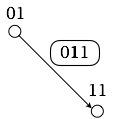
\includegraphics[scale=0.6]{FiguresGraph/dBlabelEdge}
\caption{Illustrating how to label each arc of a de Bruijn network by
  concatenating the labels of the nodes incident to the arc and
  compacting the common intermediate bits.  In the depicted example,
  the node-labels $01$ and $11$ combine to yield the arc-label $011$.}
  \label{fig:dBlabelEdge}
\end{center}
\end{figure}

\medskip

\noindent {\bf (2)}
{\it Eulerian cycles (or tours)}. \index{Eulerian cycle}
\index{Eulerian tour} A {\it directed Eulerian cycle} in a digraph
$\g$ is a directed cycle that contains each arc of $\g$ precisely
once.  We will see, later in this chapter, a truly elementary
argument, based on node-degrees, which proves that every de Bruijn
digraph has a directed Eulerian cycle.  This demonstration will
combine with Proposition~\ref{thm:deBruin-linegraph} to complete the
proof of Proposition~\ref{thm:deBruijn-Hamiltonian}.  \qed
%\end{proof}


